\chapter{AgentJ Examples}
\label{chap:examples}

\sloppypar The \agentj~example TCL scripts for running within Ns-2 can be found in the \emph{examples} directory within the \agentj~route.  The corresponding Java source code that implements these demos can be found in the \emph{src/java/agentj/examples} directory. There are several demonstration \textbf{directories} that contain the various demos AgentJ has to offer. They are:

\index{TCL Scripts}
\index{AgentJ Demonstrations}

\begin{description}
\item
\item [basic:] Contains some basic demos that show how agents are created and how commands are invoked on those agents. This directory for example contains the change delimiter demo described in the previous chapter and it also contains some demos on how to use the timers to schedule timeout triggers at certain points during the simulation.
\item [udp:] Contains a number of demos using UDP, ranging from simple client and server demos, to using multicast groups, to sending messages to multiple nodes.  
\item [tcp:] Contains some demos for creating TCP client and server sockets.  The demo simpletcp.tcl is described in more detail below.  This directory also contains a demo that combines multicast (for discovery of the nodes) and TCP for transmission of  a message (see multicastAndTcp.tcl).
\item [threads:] This directory contains demos that create Java threads for implementing the conventional way that a Java application would create a non-blocking receive() on a socket.  The demostrations show that an application can spawn multiple threads and that AgentJ keeps a track of such threads and monitors their lifetime.    One demo also shows the use of creating multiple socket threads and timers to trigger the points at which the application sends the messages, implemented using the java Thread.sleep() method.
\item [nam:] The NAM application is a visual animator for NS-2 simulations.  Typically, within the TCL script, you would insert commands in order to display labels or change colours of the nodes during the simulation.  The namdemo.tcl example here shows how to do this from within your Java application itself. This demo is described in Section \ref{sec:namdemo} 
%\item [p2ps:] Contains a number of P2PS demonstrations that use P2PS in a number of modes and configurations.  The demos range from using simple multicast discovery mechanisms to using one and multiple rendezvous peers for implementing caching mechanisms for the P2P adverts that are propagated around the network when peers join.
\item [gui:] Contains a demo that implements a graphical user interface on an Ns-2 node to poll for input.  This demonstrates the capability of allow user interactions within an Ns-2 simulation.    
\end{description}

In each directory, there is a README.TXT file, which provides an overview of each demo in that directory. The examples, described here provide a high-level illustration of just a few of the examples. It assumes that you have some knowledge of running NS-2 simulations and that you will try these demos as you read this manual for a complete picture of the TCL and Java parts of the examples.  If you are not familiar with NS-2, you will need to at least try running a few Ns-2 examples before attempting these.

 \section{TCP Socket Example}
 \label{sec:tcpdemo}

\index{AgentJ Socket Example}

In the \emph{tcp} directory, there contains a simple demo that implements the Java socket example in the Java tutorial. This demonstrates how a programmer can use the blocking Java API with the sequential nature of the NS-2 simulator.  AgentJ detects all blocking calls and creates a behind the scene non-blocking callback for such calls, which wait for data to arrive before releasing the blocked code.  Hence, a receve() call on a socket, to the Java application, simply waits (blocks) until data arrives. In AgentJ however, the call does not block, it releases control back to NS-2 and passes the control to the next node in the simulation, and waits for data asynchronously in the background.  

 \subsection{TCP Socket Example: The TCL Side}

The TCL file ``simpletcp.tcl'' can be found in the \emph{examples/tcp} directory. It simply creates two nodes with a drop tail 64kb network link connecting them.  It then creates the two Java agents and invokes commands on those agents as follows:

 \footnotesize
 \begin{verbatim}
$ns_ at 0.0 "$p1 attach-agentj agentj.examples.tcp.SimpleTCPServer"
$ns_ at 0.0 "$p2 attach-agentj agentj.examples.tcp.SimpleTCPClient"

$ns_ at 1.0 "$p1 agentj open"
$ns_ at 2.0 "$p1 agentj accept"

$ns_ at 6.0 "$p2 agentj open"
$ns_ at 10.0 "$p2 agentj send"
 \end{verbatim}
 \normalsize

\noindent Note how the ``attach-agentj'' command, described in the previous chapter is used to attach the agents.  You can attach any Java object that extends \emph{AgentJNode} to an Ns-2 node using this command.  You can then pass commands to those objects as illustrated here. In this example, we tell the server (p1) to open a server socket and then to call the accept method on that socket to wait for an incoming connection.

We then tell the client to open a socket and connect to the server and then send data to the server socket.  The result of the simulations will be something like:

\footnotesize
\begin{verbatim}
SimpleTCPServer, receing Message !!!!!!!!!!!!!!!!!!!!!!!!!!!!!!
--> Hello server, are you working?
SimpleTCPServer:: received hello message from client, sending a Reply !!!!!!!
SimpleTCPClient, receing Message !!!!!!!!!!!!!!!!!!!!!!!!!!!!!!
--> Ah, Hello client, nice to make your acquaintance...
 \end{verbatim}
 \normalsize

\noindent  As shown above, when the server socket receives the incoming message, it sends a reply to the client socket indicating that the send was successful.  The client socket receives this message and the simulation ends.  This demo is simple but shows the power of how AgentJ can run unaltered Java code.  The Java code here is trimmed replication of the Java tutorial and contains exactly the same code one would need to implement this over real world sockets.  In fact, the same Java agent code can be run outside of AgentJ to show this demo running over a real network using the Java runtime.  

 \subsection{TCP Socket Example: The Java Side}
 \label{sec:tcp:javaside}

On the java side, we have two classes:

\begin{itemize}
\item ``agentj.examples.tcp.SimpleTCPServer'' and 
\item ``agentj.examples.tcp.SimpleTCPClient'' 
\end{itemize}
\noindent found in the \emph{agentj/src/java/agentj/examples/tcp} directory. 

You can view source code directly but the example is equivalent to the Sun Java Tutorial  Knock Knock example for creating a TCP socket connection that can be found at:

\footnotesize
\begin{verbatim}
http://java.sun.com/docs/books/tutorial/networking/sockets/clientServer.html
 \end{verbatim}
 \normalsize
 
Note that in this source code, the agents simply import the java.net.* classes and write to those APIs.  This is normal for AgentJ but behind the scenes these classes are bytecode rewritten to use the AgentJ implementations of these classes.  With respect to AgentJ, the only functional difference between the Java tutorial example and the code here is to set the logging level for the Java code and C++ code. This is set in the constructor as follows: 
 
 \footnotesize
 \begin{verbatim}
setJavaDebugLevel(Level.ERROR);
setNativeDebugLevel(AgentJDebugLevel.error);        
 \end{verbatim}
 \normalsize

\noindent which indicates that only errors should be output to the stdout display.  An agent can set this level to whatever it choses.  \sloppypar AgentJ has two logging systems, one for Java and one for the C++ code.  The Java logging uses the Log4J system \cite{log4j} and the C++ code uses the Protolib logging mechanism, PLOG.     The logging levels available for each are defined in the ``org.apache.log4j.Level'' and ``AgentJNode'' classes respectively.
 

 \section{Animating NAM Demo}
 \label{sec:namdemo}
 
 \index{AgentJ NAM Demo}

This demonstration shows how add NAM display instructions from Java.  Within your Java code directly, you can change the colors of nodes, add markers, add labels and add trace messages to the NAM animations and AgentJ inserts the commands at the right point in time in the nam trace file for visualisation. This provides a very powerful annotation mechanism for simulations because often there are several message exchanges before the control comes back to TCL, so clearly annotating such messages in TCL is not enough.
Using the AgentJ NAM interface, each programmatical step can be annotated within the NAM simulation.

 \subsection{NAM Demo: The TCL Side}
 \label{jni:tclside}

This example can be found in \emph{examples/man/namdemo.tcl}. This example also shows how to attach the agents and pass commands in order to orchestrate the simulation. 

\footnotesize
\begin{verbatim}
$ns_ at 0.0 "$p1 attach-agentj agentj.examples.nam.NamDemo"
$ns_ at 0.0 "$p2 attach-agentj agentj.examples.nam.NamDemo"

$ns_ at 0.0 "$p1 agentj init-server"
$ns_ at 0.0 "$p2 agentj init-client"

$ns_ at 1.0 "$p1 agentj receive"
$ns_ at 1.0 "$p2 agentj send"
\end{verbatim}
\normalsize

\noindent The receive and send commands are repeated four times.  The resulting NAM display can be seen in Figure \ref{fig:namdemo}, which shows the nodes labelled with the  current message displayed in different colors.

\begin{figure}
\centering
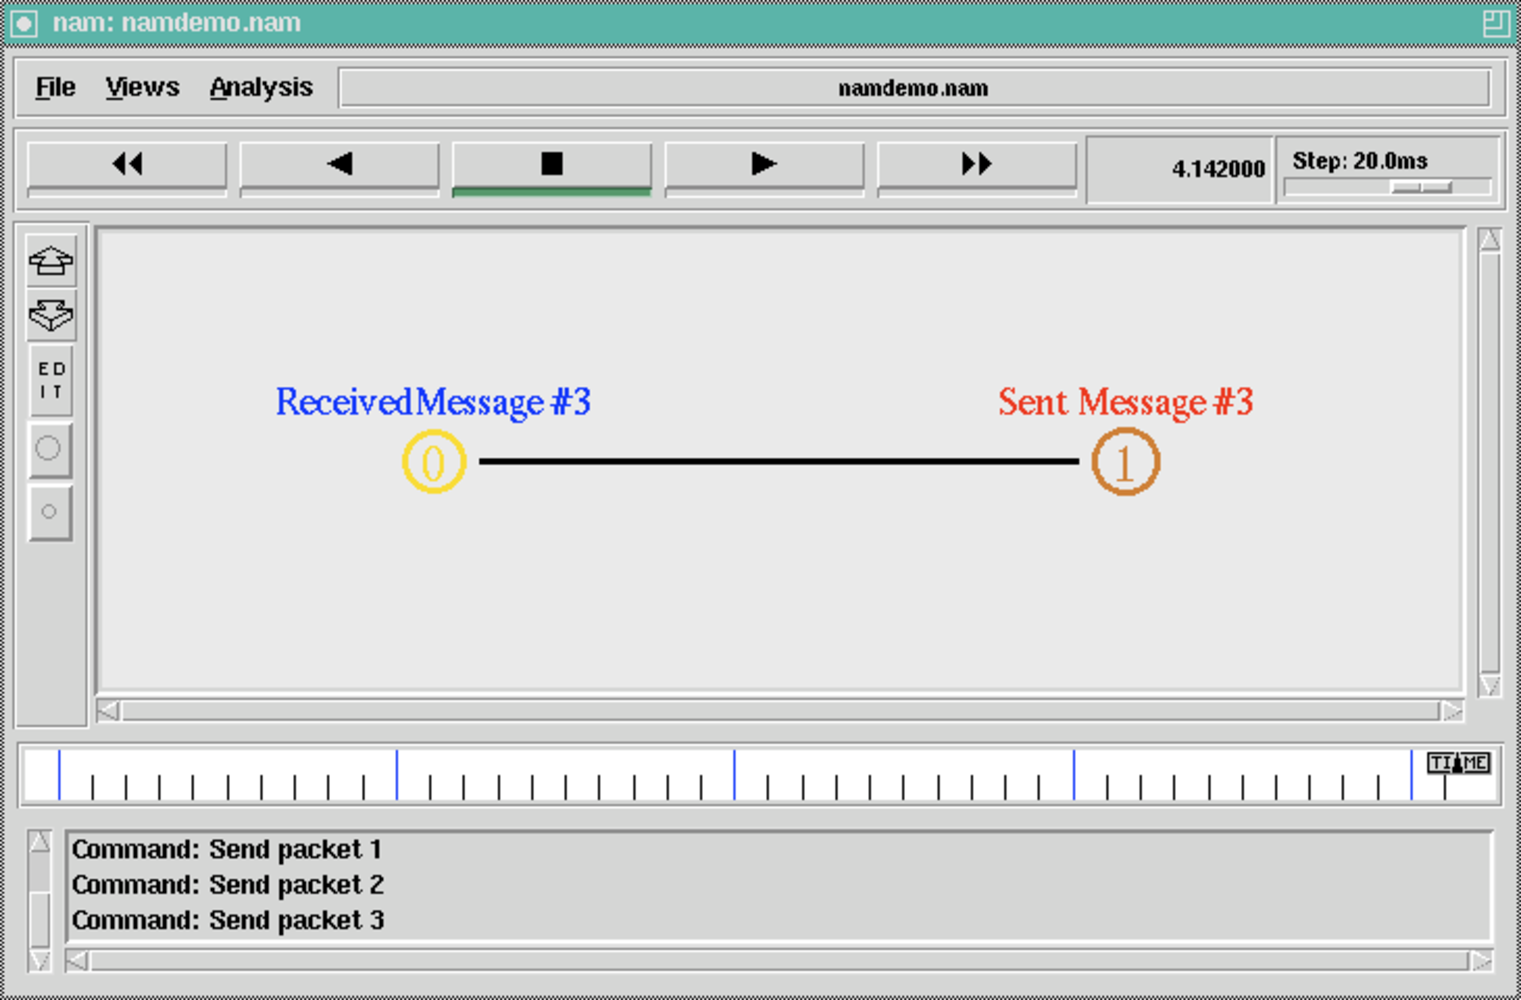
\includegraphics[scale=0.45]{images/namdemo}
\caption{The Output NAM display for the namdemo.tcl simulation}
\label{fig:namdemo}
\end{figure}
 
 \subsection{NAM Demo: The Java Side}
 \label{sec:nam:javaside}
 
 The demo actually demonstrates how to color nodes and add labels during a simulation. We use a simple multicast demo to ilustrate this. Every time a message is sent it is added as a label to the NAM animation and colors are changed. The commands are shown in the \emph{send} and \emph{receive} methods below from the NAMDemo class:

 
 \footnotesize
 \begin{verbatim}
   NAMCommands nam;

    public NamDemo() {
        this.setJavaDebugLevel(Level.DEBUG);
        this.setNativeDebugLevel(AgentJDebugLevel.detail);
        nam = this.getNamCommands();
        nam.setAnimationRate(0.02);
    }
 \end{verbatim}
 \normalsize

\footnotesize
 \begin{verbatim}
   public void send() {
        nam.setNodeColor(NAMCommands.NamColor.chocolate);
        try {
            String msg = "Message #" + msgcount;
            ++msgcount;
            DatagramPacket hi = new DatagramPacket(msg.getBytes(),msg.length(), group);
            nam.setNodeLabel("Sent " + msg, NAMCommands.LabelPosition.down, 
            							NAMCommands.NamColor.red);
            s.send(hi);
        } catch (IOException e) {
            e.printStackTrace();  
        }
    } 
 \end{verbatim}
 \normalsize

\footnotesize
 \begin{verbatim}
    public void receive() {
        nam.setNodeColor(NAMCommands.NamColor.gold);
        byte[] buf = new byte[1000];
        DatagramPacket recv = new DatagramPacket(buf, buf.length);
        try {
            s.receive(recv);
            String msg = new String(recv.getData());
            nam.setNodeLabel("Received" + msg, NAMCommands.LabelPosition.up, 
            						NAMCommands.NamColor.blue);
        } catch (IOException e) {
            e.printStackTrace(); 
        }
    }
 \end{verbatim}
 \normalsize
 
 \footnotesize
 \begin{verbatim}
 if (command.equals("send")) {
     nam.traceAnnotate("Command: Send packet " + msgcount);
     send();
 \end{verbatim}
 \normalsize


%\section{P2PS Demos}
%\label{sec:p2psdemos}

%\index{AgentJ P2PS Demonstrations}
%\index{AgentJ Peer-to-Peer Demonstrations}

%P2PS (Peer-to-Peer Simplified) \cite{p2ps} is a lightweight peer-to-peer 
%infrastructure. As the name suggests, P2PS aims to provide a simple 
%collection of middleware that a develop can use to write peer-to-peer 
%style applications, hiding the complexity of other similar architectures 
%such as JXTA~\cite{jxta} and JINI~\cite{jini2}.

%\index{JNI}

%Briefly, the P2PS infrastructure is based on XML based discovery and 
%communication, which makes it independent of any implementation 
%language and computing hardware. P2PS implementations could exist
%in any language and there is a specification which can be used to
%implement such, although at this time we have only built a prototype
%Java implementation. Furthermore, communication within P2PS is 
%not tied to any single transport protocol, such as TCP/IP, and 
%can be extended to include new protocols, such as Bluetooth or
%extend existing ones by writing new endpoint resolvers.  P2PS has 
%been designed to operate in highly dynamic, transient 
%environments and provides an overlay for discovering anything that
%a peer wants to advertise e.g. specific services, rendezvous (caching) peers,
%endpoint protocols etc.  P2PS dynamically discovers the capabilities of
%other peers at run-time and can negotiate and match how it 
%communicates and how it organises its peers.  This makes P2PS
%highly suitable for testing out different discovery mechanisms
%for two key reasons.  First, we can test the discovery mechanisms 
%built into P2PS (Multicast and Unicast) and secondly, we can easily
%extend this to include other protocols by writing new endpoint 
%resolvers. Thus, it provides a core extensible framework for testing 
%and exploring a number of mechanisms both within a simulated 
%environment or within a real-world application.

%\subsection{Simple P2PS Demos}

%This directory contains simulations using P2PS.  This work is on-going and 
%experimental, so run at your own risk :)

%\begin{enumerate}
%\item SimpleP2PS --- creates a direct UDP connection between two P2PS nodes
%\item P2PSComplex --- implements two nodes and uses multicast for discovery. Once discovered, P2PS figures out which protocols each have and negotiates a connection between them.  they connect and communicate a message.

%\end{enumerate}

%\subsection{Advanced P2PS Demos}

%These following demos use more complex network configurations and use a combination of discovery mechanisms for discovery of the nodes within the network. The network configuration consists of a client and server at the far side of the network and either zero, one, two or three rendezvous nodes in between them to aid in the discovery process. The demos use unicast or multicast depending on the mode.  Below is a brief summary of the demos:

%\begin{enumerate}
%\item P2PSMulticastDiscovery - multicast discovery demo using rendezvous nodes
%\item P2PSMulticastOneRendezvous - multicast discovery using one central independent rendezvous nodes
%\item P2PSUnicastDiscovery - unicast discovery using rendezvous nodes
%\item P2PSUnicastOneRendezvous - unicast discovery using one central independent rendezvous nodes
%\item P2PSUnicastTwoRendezvous - client and server unicast discovery using a cluster of three connected two rendezvous nodes
%\item P2PSUnicastThreeRendezvous - client and server unicast discovery using a cluster of three connected rendezvous nodes
%\end{enumerate}

%\begin{figure}
%\centering
%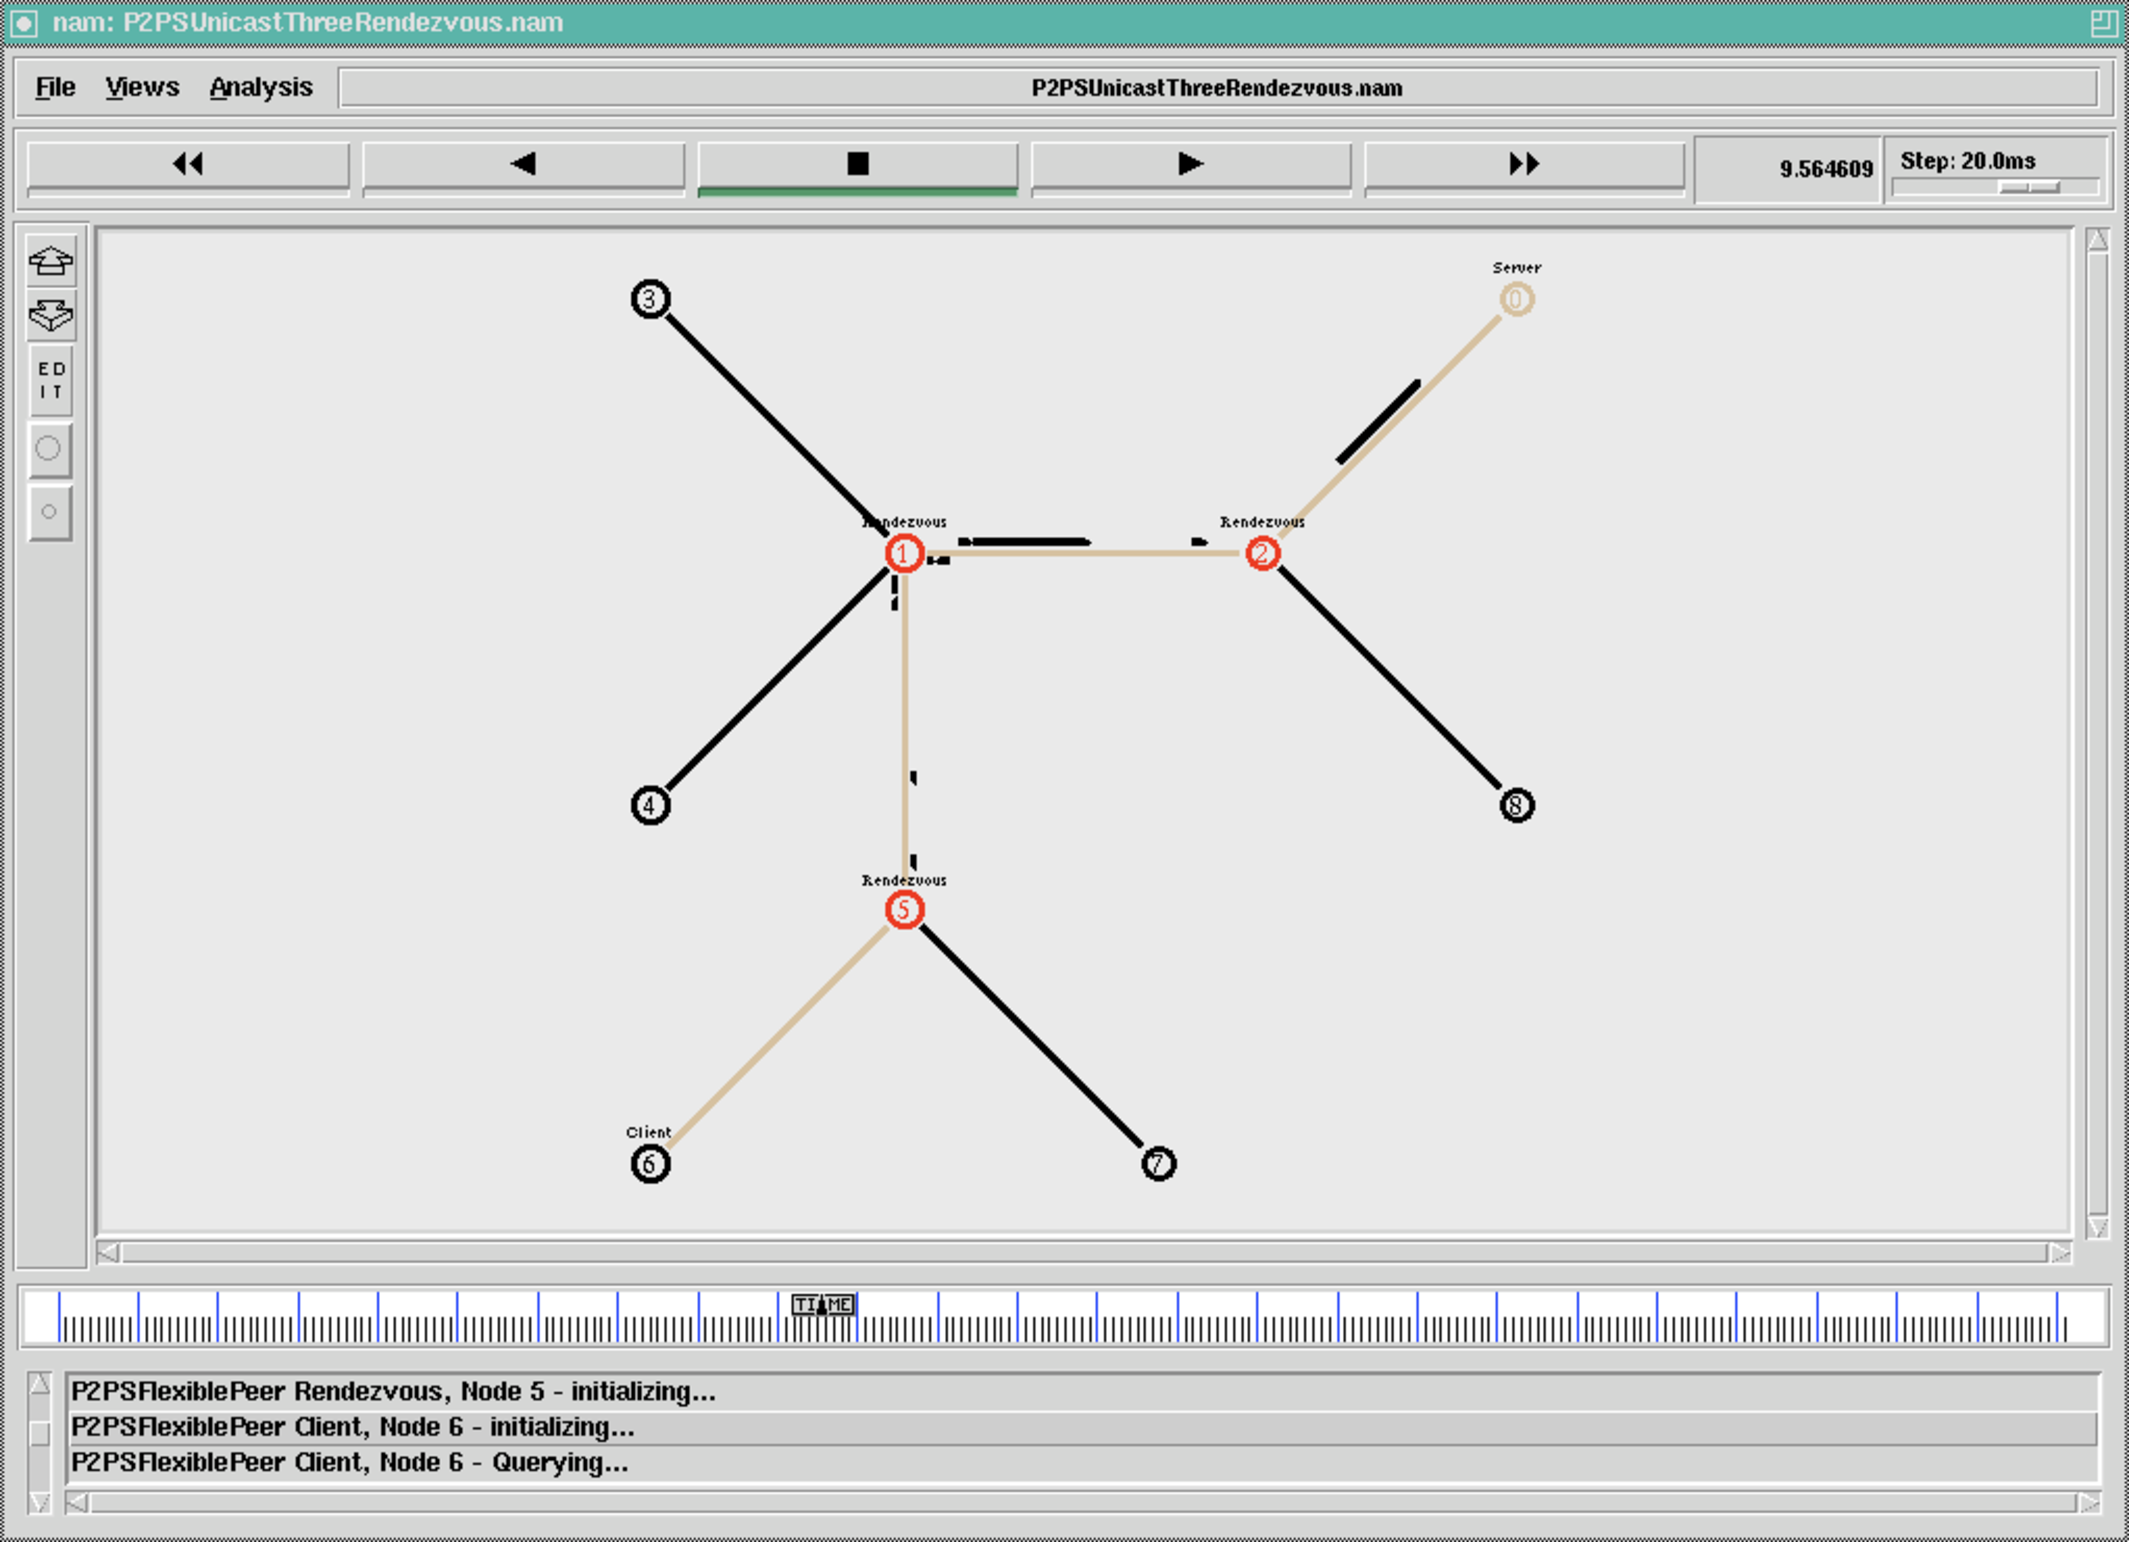
\includegraphics[scale=0.35]{images/p2psdemo}
%\caption{The network configuration for the Unicast Three Rendezvous P2PS demo.}
%\label{fig:p2psdemo}
%\end{figure}

%Figure \ref{fig:p2psdemo} shows a snapshot of a P2PS simulation.  In this example, there are three rendezvous peers in the center of the network, which are accessed by the client and server on the far sides.  The black segments show the data flow between the nodes during this time-slice of this simulation, and their length indicates the size of that data packet.  \noindent Go ahead and try these out yourself, you can find them in \emph{src/java/agentj/examples/p2ps}.

